\section{Database Design}
\label{sec:database-design}

\subsection{Technology and conventions}
\status{IMPLEMENTED}

\begin{table}[H]
\centering
\caption{Database technology and design conventions}
\label{tab:db-facts}
\begin{tabular}{@{}L{4.4cm}L{9.8cm}@{}}
\toprule
\textbf{Aspect} & \textbf{Fact (evidence)} \\
\midrule
Engine & MySQL 8, InnoDB, \code{utf8mb4_unicode_ci} (\pathref{database/schema.sql}) \\
Test engine & H2 in-memory, \code{MODE=MySQL}, \code{ddl-auto: create-drop} (\pathref{backend/src/main/resources/application-test.yml}) \\
Schema authority & \pathref{database/schema.sql} (hand-authored) + Hibernate \code{ddl-auto: update} at startup \\
Identifier strategy & \code{BIGINT AUTO_INCREMENT} primary keys (no UUIDs) \\
Timestamps & \code{created_at}/\code{updated_at} defaults, \code{ON UPDATE CURRENT_TIMESTAMP} \\
Soft delete & Enrolments use status \code{DROPPED}; courses/users are hard-deleted \\
Naming & snake\_case tables/columns; JPA maps via naming strategy \\
Table count & 13 tables \\
\bottomrule
\end{tabular}
\end{table}

\subsection{Entity-relationship diagram}
\status{IMPLEMENTED}

\begin{figure}[H]
    \centering
    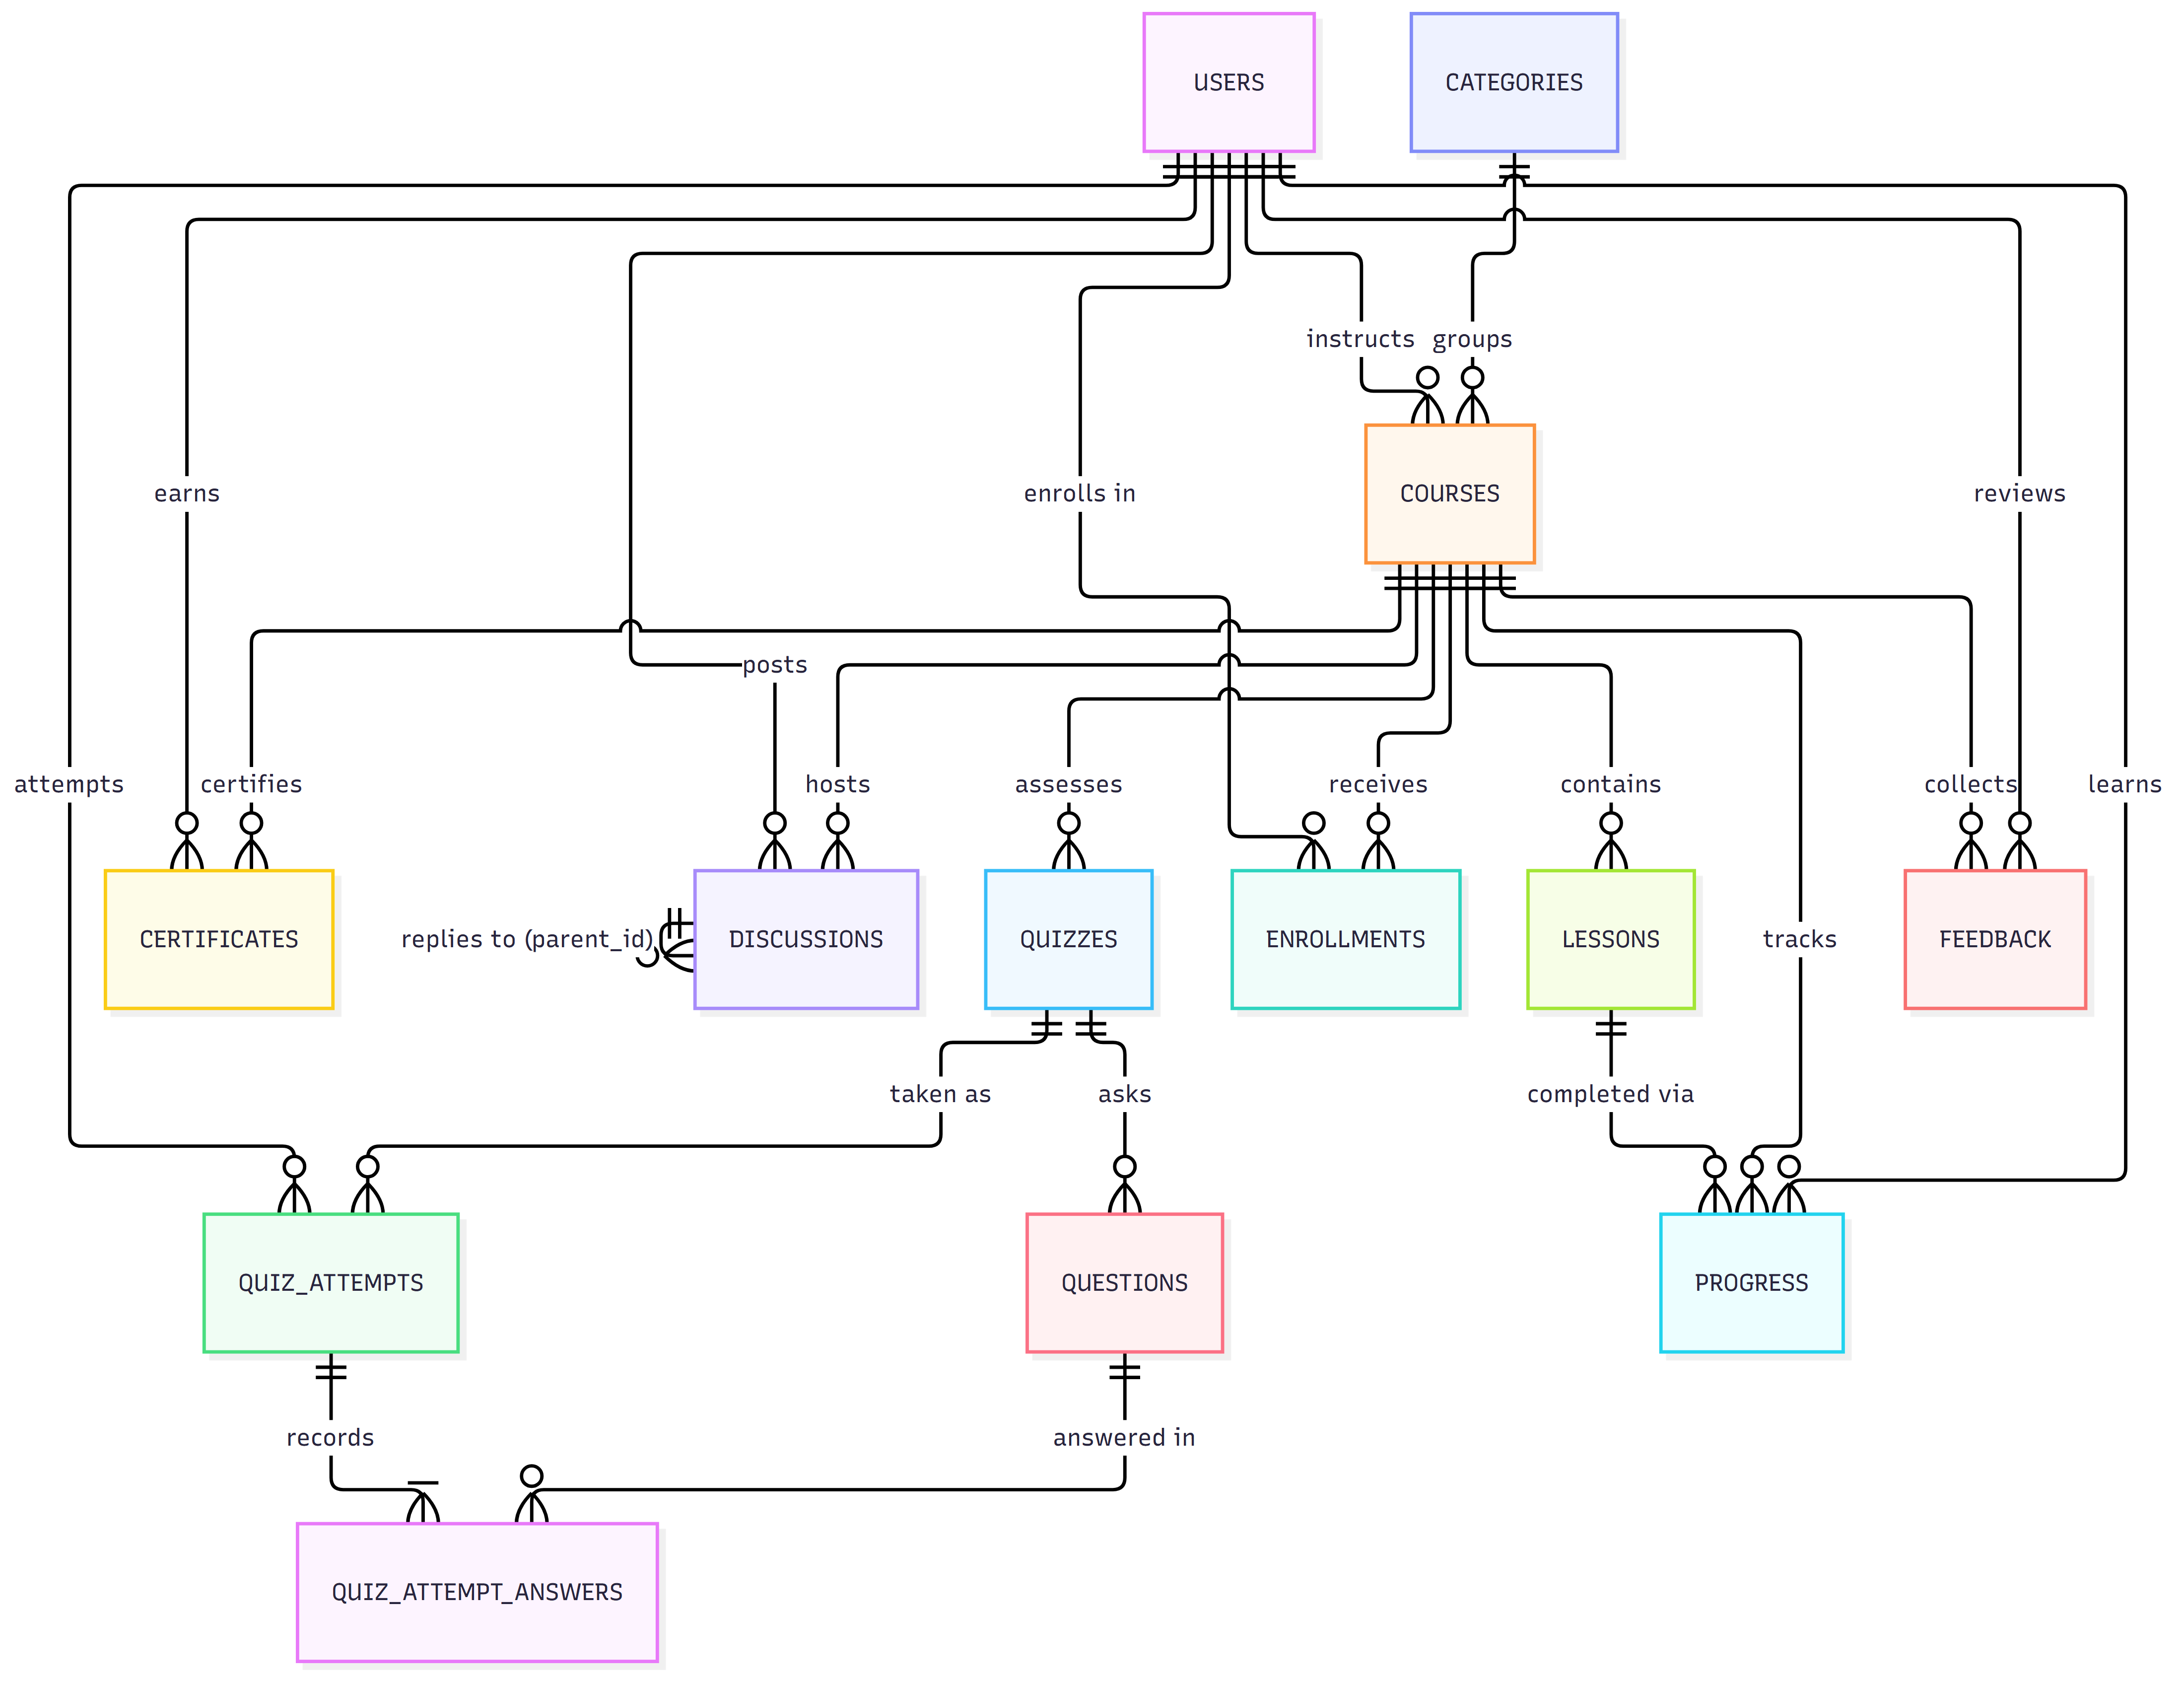
\includegraphics[width=\textwidth]{diagrams/database-er.png}
    \caption{Entity-relationship diagram of the 13 LMS tables}
    \label{fig:database-er}
\end{figure}

\subsection{Tables}
\status{IMPLEMENTED}

\subsubsection{users}
\begin{lstlisting}[language=sql,caption={users table (database/schema.sql)}]
id BIGINT PK AUTO_INCREMENT
name VARCHAR(100) NOT NULL
email VARCHAR(150) NOT NULL UNIQUE          -- idx_users_email
password VARCHAR(255) NOT NULL              -- BCrypt hash
role VARCHAR(30) NOT NULL DEFAULT 'LEARNER' -- idx_users_role
bio TEXT NULL
avatar_url VARCHAR(512) NULL
created_at, updated_at TIMESTAMP NOT NULL DEFAULT CURRENT_TIMESTAMP
\end{lstlisting}

\subsubsection{categories}
\begin{lstlisting}[language=sql]
id BIGINT PK
name VARCHAR(100) NOT NULL UNIQUE
description TEXT NULL
created_at, updated_at TIMESTAMP ...
\end{lstlisting}

\subsubsection{courses}
\begin{lstlisting}[language=sql]
id BIGINT PK
title VARCHAR(255) NOT NULL
description TEXT NULL
category_id BIGINT NULL  -> categories(id) ON DELETE SET NULL   -- fk_courses_category
instructor_id BIGINT NOT NULL -> users(id) ON DELETE CASCADE   -- fk_courses_instructor
status VARCHAR(30) NOT NULL DEFAULT 'DRAFT'                    -- idx_courses_status
thumbnail_url VARCHAR(512) NULL
-- indexes: idx_courses_instructor, idx_courses_category
\end{lstlisting}

\subsubsection{lessons}
\begin{lstlisting}[language=sql]
id BIGINT PK
course_id BIGINT NOT NULL -> courses(id) ON DELETE CASCADE      -- fk_lessons_course
title VARCHAR(255) NOT NULL
description TEXT NULL
content_url VARCHAR(512) NULL        -- video / external resource
content_text LONGTEXT NULL           -- written lesson body
order_index INT NOT NULL DEFAULT 1   -- idx_lessons_order (course_id, order_index)
duration_minutes INT NOT NULL DEFAULT 0
created_at, updated_at TIMESTAMP ...
\end{lstlisting}

\subsubsection{enrollments}
\begin{lstlisting}[language=sql]
id BIGINT PK
user_id BIGINT NOT NULL -> users(id) ON DELETE CASCADE
course_id BIGINT NOT NULL -> courses(id) ON DELETE CASCADE
status VARCHAR(30) NOT NULL DEFAULT 'ENROLLED'  -- ENROLLED|COMPLETED|DROPPED
enrolled_at TIMESTAMP NOT NULL DEFAULT CURRENT_TIMESTAMP
completed_at TIMESTAMP NULL
UNIQUE KEY uk_user_course_enrollment (user_id, course_id)
-- indexes: idx_enrollments_user, idx_enrollments_course, idx_enrollments_status
\end{lstlisting}

\subsubsection{progress}
\begin{lstlisting}[language=sql]
id BIGINT PK
user_id BIGINT NOT NULL -> users(id) ON DELETE CASCADE
course_id BIGINT NOT NULL -> courses(id) ON DELETE CASCADE
lesson_id BIGINT NOT NULL -> lessons(id) ON DELETE CASCADE
completed BOOLEAN NOT NULL DEFAULT FALSE
watch_time_seconds INT NOT NULL DEFAULT 0
completion_percentage DOUBLE NOT NULL DEFAULT 0.0
updated_at TIMESTAMP ...
UNIQUE KEY uk_user_lesson_progress (user_id, lesson_id)
INDEX idx_progress_user_course (user_id, course_id)
\end{lstlisting}

\subsubsection{quizzes}
\begin{lstlisting}[language=sql]
id BIGINT PK
course_id BIGINT NOT NULL -> courses(id) ON DELETE CASCADE
title VARCHAR(255) NOT NULL
description TEXT NULL
passing_score INT NOT NULL DEFAULT 70
time_limit_minutes INT NOT NULL DEFAULT 30
created_at, updated_at TIMESTAMP ...
INDEX idx_quizzes_course (course_id)
\end{lstlisting}

\subsubsection{questions}
\begin{lstlisting}[language=sql]
id BIGINT PK
quiz_id BIGINT NOT NULL -> quizzes(id) ON DELETE CASCADE
question_text TEXT NOT NULL
option_a..option_d VARCHAR(500) NOT NULL      -- four fixed options
correct_option VARCHAR(10) NOT NULL           -- 'A'..'D'
points INT NOT NULL DEFAULT 10
explanation TEXT NULL
created_at, updated_at TIMESTAMP ...
INDEX idx_questions_quiz (quiz_id)
\end{lstlisting}

\subsubsection{quiz\_attempts} and \subsubsection{quiz\_attempt\_answers}
\begin{lstlisting}[language=sql]
quiz_attempts:
  id BIGINT PK
  quiz_id BIGINT NOT NULL -> quizzes(id) ON DELETE CASCADE
  user_id BIGINT NOT NULL -> users(id) ON DELETE CASCADE
  score INT DEFAULT 0, total_points INT DEFAULT 0, passed BOOLEAN DEFAULT FALSE
  started_at TIMESTAMP NOT NULL, submitted_at TIMESTAMP NULL
  indexes: idx_quiz_attempts_user, idx_quiz_attempts_quiz

quiz_attempt_answers:
  id BIGINT PK
  attempt_id BIGINT NOT NULL -> quiz_attempts(id) ON DELETE CASCADE
  question_id BIGINT NOT NULL -> questions(id) ON DELETE CASCADE
  selected_option VARCHAR(10) NOT NULL
  is_correct BOOLEAN DEFAULT FALSE, points_awarded INT DEFAULT 0
  index: idx_attempt_answers_attempt
\end{lstlisting}

\subsubsection{discussions}
\begin{lstlisting}[language=sql]
id BIGINT PK
course_id BIGINT NOT NULL -> courses(id) ON DELETE CASCADE
user_id BIGINT NOT NULL -> users(id) ON DELETE CASCADE
parent_id BIGINT NULL -> discussions(id) ON DELETE CASCADE   -- self reference (threads/replies)
title VARCHAR(255) NULL       -- NULL for replies
content TEXT NOT NULL
created_at, updated_at TIMESTAMP ...
indexes: idx_discussions_course, idx_discussions_parent
\end{lstlisting}

\subsubsection{feedback}
\begin{lstlisting}[language=sql]
id BIGINT PK
course_id BIGINT NOT NULL -> courses(id) ON DELETE CASCADE
user_id BIGINT NOT NULL -> users(id) ON DELETE CASCADE
rating INT NOT NULL CHECK (rating >= 1 AND rating <= 5)
comment TEXT NULL
created_at, updated_at TIMESTAMP ...
UNIQUE KEY uk_user_course_feedback (user_id, course_id)
INDEX idx_feedback_course (course_id)
\end{lstlisting}

\subsubsection{certificates}
\begin{lstlisting}[language=sql]
id BIGINT PK
certificate_code VARCHAR(64) NOT NULL UNIQUE    -- idx_certificates_code
user_id BIGINT NOT NULL -> users(id) ON DELETE CASCADE
course_id BIGINT NOT NULL -> courses(id) ON DELETE CASCADE
issue_date TIMESTAMP NOT NULL DEFAULT CURRENT_TIMESTAMP
grade VARCHAR(50) DEFAULT 'PASS'                -- runtime value is 'DISTINCTION'
certificate_url VARCHAR(512) NULL               -- API path to the certificate
UNIQUE KEY uk_user_course_certificate (user_id, course_id)
\end{lstlisting}

\subsection{Relationship summary}
\status{IMPLEMENTED}

\begin{table}[H]
\centering
\caption{Foreign-key relationships and cardinalities}
\label{tab:relationships}
\begin{tabular}{@{}L{3.6cm}L{3.6cm}C{2.4cm}L{4.0cm}@{}}
\toprule
\textbf{Child} & \textbf{Parent} & \textbf{Cardinality} & \textbf{On delete} \\
\midrule
courses.category\_id & categories & optional many--one & SET NULL \\
courses.instructor\_id & users & many--one (required) & CASCADE \\
lessons.course\_id & courses & many--one & CASCADE \\
enrollments.user\_id / course\_id & users / courses & many--many (associative) & CASCADE \\
progress.user\_id / course\_id / lesson\_id & users / courses / lessons & many--one per dimension & CASCADE \\
quizzes.course\_id & courses & many--one & CASCADE \\
questions.quiz\_id & quizzes & many--one & CASCADE \\
quiz\_attempts.quiz\_id / user\_id & quizzes / users & many--one & CASCADE \\
quiz\_attempt\_answers.attempt\_id / question\_id & quiz\_attempts / questions & many--one & CASCADE \\
discussions.parent\_id & discussions & self (thread/reply) & CASCADE \\
feedback.course\_id / user\_id & courses / users & many--one & CASCADE \\
certificates.user\_id / course\_id & users / courses & many--one & CASCADE \\
\bottomrule
\end{tabular}
\end{table}

\subsection{Indexes and constraints}
\status{IMPLEMENTED}

\begin{itemize}
    \item \textbf{20 secondary indexes} declared in \pathref{database/schema.sql} (email, role, instructor, category, status, course lookups, user/course pairs, attempt/answer lookups, discussion parent, certificate code).
    \item \textbf{4 unique business keys:} \code{uk_user_course_enrollment}, \code{uk_user_lesson_progress}, \code{uk_user_course_feedback}, \code{uk_user_course_certificate} -- these enforce ``one enrolment / one progress row / one review / one certificate'' at the database level.
    \item \textbf{Check constraint:} \code{feedback.rating} between 1 and 5 (schema-level; additionally enforced by \code{@Min(1)}/\code{@Max(5)} on the DTO).
    \item \textbf{Referential deletion:} child rows cascade with their parents; removing a category only detaches courses.
\end{itemize}

\subsection{Views, stored procedures, functions, triggers}
\status{NOT APPLICABLE (verified)}

\pathref{database/schema.sql} contains no \code{VIEW}, \code{PROCEDURE}, \code{FUNCTION} or \code{TRIGGER} statements; all derived values (progress percentages, counts, scores) are computed in the application layer.

\subsection{Row-level security and database access control}
\status{NOT IMPLEMENTED / NOT APPLICABLE}

MySQL has no RLS feature; the repository configures no dedicated database roles or grants (the app connects with credentials from the datasource configuration, defaulting to \code{root}). All row-level enforcement happens in Java services. \status{RECOMMENDED} a least-privilege application DB user for production.

\subsection{Migrations and schema evolution}
\status{PARTIAL}

\begin{itemize}
    \item No Flyway or Liquibase dependency exists in \pathref{backend/pom.xml}; there are no versioned migration files.
    \item Schema is created by \pathref{database/schema.sql} (manual import, documented in \pathref{README.md}) and then kept in sync by Hibernate \code{ddl-auto: update}, which can add tables/columns but never alters or drops them.
    \item \pathref{database/seed.sql} and \pathref{database/dummy.sql} provide \code{INSERT IGNORE} sample data (demo users with BCrypt hash for \code{password123}, 2--3 sample courses, lessons, quizzes, questions).
\end{itemize}
\noindent \textbf{Risk:} schema drift between hand-written SQL and entity definitions is possible and untested in CI (no pipeline). See Section~\ref{sec:technical-debt}.

\subsection{Entity/schema parity notes}
\status{IMPLEMENTED (observations)}

\begin{itemize}
    \item All 13 \code{@Entity} classes map one-to-one to the 13 tables (verified: \code{@Table} names match).
    \item The runtime \code{grade} value written by \code{CertificateService} is \code{DISTINCTION} while the column default is \code{PASS} -- cosmetic inconsistency documented in Section~\ref{sec:known-issues}.
    \item The \code{progress} table has no \code{created_at} (only \code{updated_at}) -- matches the entity.
\end{itemize}
